\chapter{再读德鲁克 从管理外包人员到全面质量管理} % Introduction chapter suppressed from the table of contents

\framebox{%
\begin{minipage}[t]{0.97\columnwidth}\raggedright
有一家电力行业的软件开发部,因为要控制全职员工的人数,所以很多开发人员都是以外包形式聘用,以下这个表是我们抽看的三个项目的数据,第一列是这个项目的功能点数,倒数第二列是项目的缺陷数。


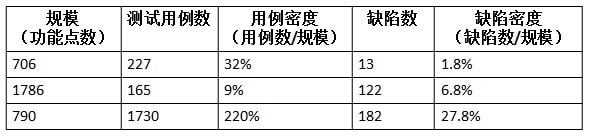
\includegraphics[width=8cm]{Druker_6_外包管理_1.jpg}

可以看出,项目的缺陷密度差异很大。与第一个项目团队沟通,发现写完代码没有单元测试,也没有评审代码,所以估计系统测试缺陷密度这么低,并不表示代码质量好,只是测试力度不够(项目1本来报给我的测试用例数是34,后来再说227才对)。\strut
\end{minipage}}

从以上的例子,就看到如果项目管理不善,质量问题可以很严重。

下面我们先回顾德鲁克先生2002年"They are not Employees,they are
people"文章{[}1{]}的重点,然后再探讨管理者如何提高知识工作者的质量与生产率。

\hypertarget{ux4e34ux65f6ux5de5temp-ux4e0e-ux4e13ux4e1aux96c7ux4e3bux7ec4ux7ec7}{%
\subsection{临时工(Temp) 与
专业雇主组织}\label{ux4e34ux65f6ux5de5temp-ux4e0e-ux4e13ux4e1aux96c7ux4e3bux7ec4ux7ec7}}

临时工(Temp)这行业早在50年代开始崛起,开始的时候主要负责一些简单岗位:文员、前台、电话操作员等,后来慢慢扩大到各种岗位,甚至总裁都有临时工。\\
\textbf{专业雇主组织 Professional employee organization (PEO)}\\
曾经,有顾问公司统计过一般公司管理员工的成本,约占总成本的25\%\textasciitilde{}30\%,所以如果有公司可以帮企业省去这部分成本,企业肯定愿意。这就是PEO公司的商业模式,它在90年代快速崛起,主要为客户提供企业管理人员,包括行政、人事等。\\
这两类公司为企业创造什么价值?为什么这么受欢迎?\\
德鲁克先生用一个小型医院为例:
一家有三百个病床规模的医院,大概有3000员工。其中有一半多是专业的知识工作者,除了医生、护士外、还有其他很多辅助角色:如物理治疗、化验、X光等专业岗位,但在这类医院里,每个专业可能只需要几位。医院的主管也不可能每个专业都懂,他如何管理手下各种专业人员呢?而且由于每个专业的人数不多,升迁的机会也几乎是零。例如,这医院的化验室专员全院只有三位,没有任何上升机会。但如果这些专业人员是受聘于PEO外包公司,有能力化验人员可能会被调到一些更大的医院去。而这些人也愿意用这种形式去服务医院。\\
这种现象也不仅仅适用于医院,一些百货公司、金融服务公司也常用这种方式,以获得专业性强的员工。所以这种无论临时工公司或者PEO公司,无论对员工或者雇主都有价值和吸引力。\\
这些Temp供应商 和 PEO
说能帮助企业管理员工,提升效率。你相信吗?让我们先听听大陆软件开发的管理者
和 临时工的 心声:

\hypertarget{ux5916ux5305ux95eeux9898}{%
\subsection{外包问题}\label{ux5916ux5305ux95eeux9898}}

\framebox{%
\begin{minipage}[t]{0.97\columnwidth}\raggedright
某北京IT总监的外包心得分享:\\
1. 外包的主因是降低风险\\
2. 用人员外包控制员工数量\\

\begin{itemize}
\tightlist
\item
  外包主要选我们没有它们的技术(外包公司可以提供此技术或产品或软件开发),一般考量是他们是否已做过\\
\item
  外包人员加入到我们的开发团队onsite人员,一起工作\\
\item
  问题主要是怎么调动人员积极性\\
\end{itemize}
\strut
\end{minipage}}

不少企业为了控制全职员工人数,会把软件开发项目外包出去。\\
但承包商人员水平与积极性难以保证,很可能导致软件质量出问题。\\
部分公司内IT员工的心声:\\
*\textbf{通过外包途径招聘人员的技能、质量不太能够符合项目要求,需要花费大量时间、精力去做培训,希望公司招聘外包人员时,考虑人员质量,解决项目实际人员需求。}\\
*\textbf{外包公司写的代码质量与我们自己写的相差甚远,也没有做单元测试,没有做静态代码检测,写完代码也没有做人工走查,导致我们后面很多返工。}\\
部分外包承包商员工的心声:\\
*\textbf{最大的问题是项目成就/责任感低,能少做的尽量不多做。因太多因素影响项目总体成败,我们(承包商)认为只要完成SOW里的内容就算项目成功。}\\
*\textbf{虽然公司经常组织学习甲方的产品,培训考试,项目质量主要由发包商项目经理(PM)控制,我们对项目质量关注度少,主要听PM安排。}\\
{[}SOW=Statement Of Work 可简单理解成项目需求范围 {]}\\

\hypertarget{ux77e5ux8bc6ux5de5ux4f5cux8005-ux4e0e-ux7cfbux7edf}{%
\subsection{知识工作者 与
系统}\label{ux77e5ux8bc6ux5de5ux4f5cux8005-ux4e0e-ux7cfbux7edf}}

``现代企业都依赖知识型团队, 比较50年前以劳工为主的企业,
更需要关注每一个员工的健康成长。 知识工作者最能为公司产生价值。
甚至企业的成败也依赖于知识工作者的表现。

企业不可能大量招聘卓越的人,所以管理者的挑战是如何使普通人做出超凡的事。好比杰出的指挥家能领导一普通乐团演奏出非凡的乐章。''\\
公司的创新大部分依赖于知识工作者,所以我们无论是用外包形式或者正常聘用,知识工作者是企业的核心资源(capital)。\\
以前的工业时代,是劳动者支撑系统制造产品,在当今的知识型社会恰恰相反,企业系统要支持知识工作者,让他们能发挥效益。

从外包人员的心声,和其产出软件的质量,都能觉得他们当中的很多人缺乏积极性。
所以不要以为单靠加强培训就会有效果。

具体有什么方法呢?

\framebox{%
\begin{minipage}[t]{0.97\columnwidth}\raggedright
一家工厂舍弃了传送带生产方式,学习丰田生产方式(Toyota Production System
TPS),权力下放给一线员工。企业总工有以下感想:\\

\texttt{..去巡视生产现场的时候,有一位女员工对我说:"以前每一次往生产线跟前一坐,我满脑子就都是怎么还不到5点呢?但现在上班成为一件让人高兴的事。"~听了她的话以后,我更加相信生产改革的方向没有走错。..}~\\
\strut
\end{minipage}}

为什么丰田生产方式这"系统"能改变生产现场员工的积极性?

\hypertarget{ux4e30ux7530ux6545ux4e8b}{%
\subsubsection{丰田故事}\label{ux4e30ux7530ux6545ux4e8b}}


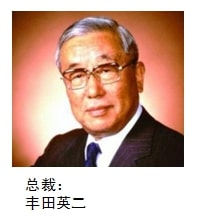
\includegraphics[width=8cm]{丰田总裁.jpg}


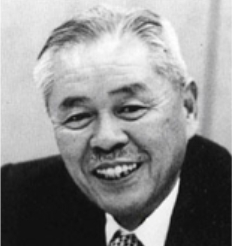
\includegraphics[width=8cm]{大野耐一.jpg}

二战后50年代,丰田汽车规模很小,经营很困难,在破产边缘。
但丰田英二先生明白美国批量生产线的弊端,意识到未来的汽车生产必须是Just-In-Time::

\begin{itemize}
\tightlist
\item
  每一辆都是按客人订单订制:例如,颜色,配置,左右钛等
\item
  从钢材原料开始,整个生产线,零等待,零浪费
\end{itemize}

\begin{description}
\item[]
\begin{description}
\tightlist
\item[]
每个工作步骤所需配件按生产需要到达
(不晚,也不早到),把生产过程中的配件降到零
\end{description}
\end{description}

安排总工大野耐一去美国汽车公司考察,
他从美国的超市(非汽车公司)得到如何做Just-In-Time的启发。
回国后就开始在丰田致力推动。


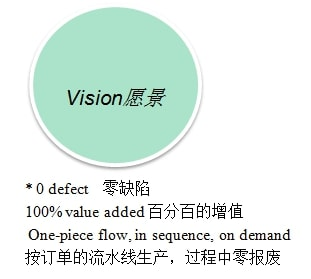
\includegraphics[width=10cm]{远景1.jpg}

开始时,很多人都觉得这个愿景好像是远不可及的梦想。今天Just-In-Time已成为汽车制造的主流,例如:日产在英国牛津(Oxfordshire)专门生产mini
车的 工厂便能做到:

\begin{itemize}
\tightlist
\item
  从钢材原料到生产出汽车只需要24小时
\item
  整个生产线没有任何中间等候,每68秒出一辆
\item
  每天生产1000辆车
\end{itemize}

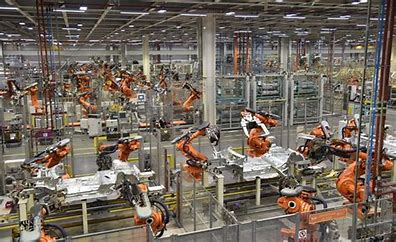
\includegraphics[width=10cm]{NissanRobots-OIP_h8UAC7FBjlaCmA_mBepJjQHaEi.jpg}

\textbf{挑战}:每一辆汽车都不同 -- 颜色,设备,左右驾驶座等

\begin{itemize}
\tightlist
\item
  生产线上每一辆汽车都按照客户需求订制
\item
  组件不早不晚按需求准时到达生产线
\item
  这便需要信息化系统把客户订单转换成生产信息
\end{itemize}


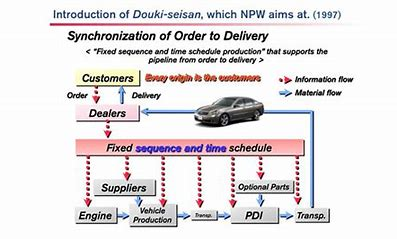
\includegraphics[width=10cm]{NissanJIT_OIP_RQGKy67DWGTu-DQiOCqW2gHaEK.jpg}
例如,生产线上每一辆的颜色都可以不同:\\

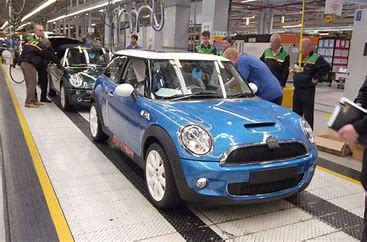
\includegraphics[width=10cm]{NissanProdLineOIP_wJFmfMl7q2_V8JaQi4kQ8QHaE6.jpg}\\


\hypertarget{ux7ba1ux7406ux5916ux5305ux4ebaux5458ux7684ux6311ux6218}{%
\subsection{管理外包人员的挑战}\label{ux7ba1ux7406ux5916ux5305ux4ebaux5458ux7684ux6311ux6218}}



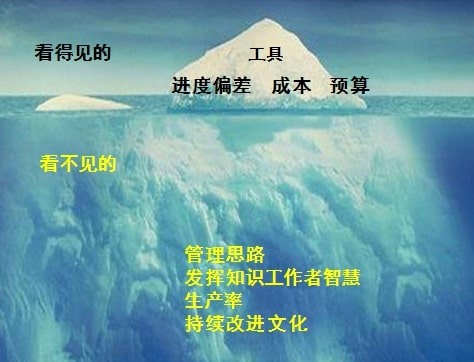
\includegraphics[width=10cm]{冰山.jpg}

\textbf{问}:我们不是讨论如何管理软件开发外包人员吗?为什么转到讨论丰田生产方式?
我们都不是生产业,有什么关系?\\
\textbf{答}:德鲁克先生2002年的文章强调:不能依赖外包公司帮你管理,
还是必须靠管理者自己。

很多软件开发公司缺乏相关度量。
例如,只管项目有没有延误,客户有没有投诉等水面上看得见的东西;但不知道生产率(每人每天生多少功能点)/现在是什么水平等水面以下看不见的情况。
没有度量就无法谈改进,无法管理。

管理者也不能仅看表面的数据,如项目延误,成本是否超支,更需要看过程中知识工作者的生产率和质量是否有提升。

外包人员每天工作都是被动地应付客户的投诉;
只想被安排的任务不延误,不会想怎样提升整个开发的效率与质量。
工作自然没有动力。

反过来,如果大家都知道自己的生产率水平, 像丰田有具体的阶段改进目标。
管理者辅导团队如何利用智慧,找出问题的根因,实施应对措施,看能否达到预期提高(而不是靠喊`要努力,努力')。
公司便可以生产出更多新产品,使客户满意,增加收入,
公司根据各团队贡献,鼓励团队分享成果,形成持续改进(PDCA)良性循环。

有这类``系统''才能根治外包人员的管理问题。

为什么丰田能成功地把汽车生产做到 Just-In-Time
,超越西方的巨头,使日本汽车制造过程成为世界"标准"?
但我们不能单从表面看这"系统"的方法和技巧,例如大家都熟悉的看板管理(他的竞争对手通用、福特、肯定都学过),所以更重要是了解背后的管理思路:\\

\hypertarget{ux4ee5ux5fd9ux788cux4e3aux803b}{%
\subsubsection{以忙碌为耻}\label{ux4ee5ux5fd9ux788cux4e3aux803b}}

\begin{itemize}
\tightlist
\item
  不吝惜智慧,但要吝惜汗水
\end{itemize}

\framebox{%
\begin{minipage}[t]{0.97\columnwidth}\raggedright
{把``动作''转变为 ``工作''}
以前,当大家批评某机关的工资太高时,职员会以上班时间很长,
``一直在努力工作''为由来反驳人们的批评。这其实是一种对于``有动作''和``在工作''的混淆。不管上班时间有多长,如果没能够创造出利润,那么就不能称之为工作,也不能称之为一直在努力。
丰田是把``动作''和``工作''分开考虑的。\\
strut 在丰田看来,
``就算一直在动也不代表那个人在工作''。
省掉徒劳动作,把``在动着''转化为``在工作''。\\
大野耐一先生曾经问过年轻员工:
``每天工作一小时左右,你们能做到吗?"
听了这句话后,有人抱怨``算上加班时间,我们一天工作九个小时,他那句话是什么意思?"确实,他们在公司待了很长时间,但如果把``有动作''和``在工作''分开考虑,九个小时中,真正在工作的时间可能只有一小时。大野先生指的是这一点。\\
关键的不在于流着汗在公司转了多长时间,而要把自己的工作区分成``徒劳作业''和``有价值作业''。\\
\strut
\end{minipage}}

因缺乏数据,很难判断这些软件开发人员每天有效生产多少?什么因素妨碍员工生产率提升?\\

\framebox{%
\begin{minipage}[t]{0.97\columnwidth}\raggedright
二战后,日本经济萎缩,丰田辞退了不少员工;1950年,朝鲜战争,需要大量增产,但丰田选择了只增加设备,而不增加人手,大野先生也借这机会,完善丰田生产方式,成功找到了以不增加人手为前提的增产办法。
\strut
\end{minipage}}

在软件开发行业,跟当年丰田一样,也会因市场的起落导致景气或不景气。很多公司预计到项目量增加就立马增聘开发、测试人手,而不是基于现有人力,如何更好利用自动化来提高生产率。我们看很多公司也是因为测试团队天天都说人手不够,增聘测试人员,反而妨碍了公司推动测试自动化。\\

\hypertarget{ux57f9ux517bux4ebaux624d---ux903cux4ed6ux4eecux52a8ux8111ux7b4b}{%
\subsubsection{培养人才 -
逼他们动脑筋}\label{ux57f9ux517bux4ebaux624d---ux903cux4ed6ux4eecux52a8ux8111ux7b4b}}

\framebox{%
\begin{minipage}[t]{0.97\columnwidth}\raggedright{人了不起的智慧}
所谓丰田生产方式其实就是要建立起一种体制,把``人了不起的智慧''引导出来,使得这些智慧能在生产一线得到充分发挥。所以说``丰田生产方式源自人的智慧''。\strut
\end{minipage}}

企业相信员工的智慧以后,员工们的干劲、使命感、责任感都会随之而生,最重要的是,员工们会因此逐渐对工作抱有自豪感。一旦员工们的意识改变了,理所当然地,企业的竞争力也将获得很大的提高。\\
丰田生产方式是TQM (Total Quality
Management全面质量管理)的最佳例子,TQM强调专注客户、持续改进、以数据说话、员工参与等,丰田生产方式覆盖了
TQM 原则的 七项 (除了战略)


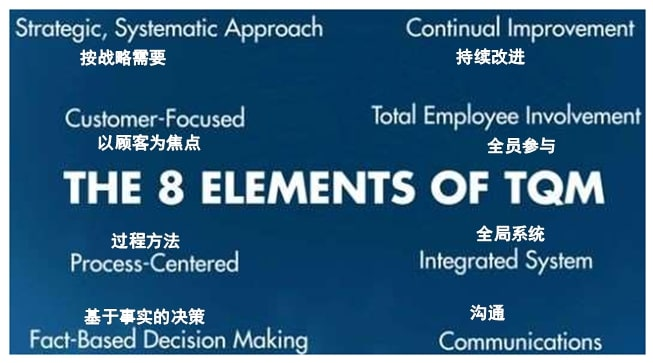
\includegraphics[width=10cm]{TQM_1_2.jpg}

\hypertarget{ux4eceux5fc3ux91ccux76f8ux4fe1ux5927ux5bb6ux7684ux529bux91cf}{%
\subsubsection{从心里相信``大家的力量''}\label{ux4eceux5fc3ux91ccux76f8ux4fe1ux5927ux5bb6ux7684ux529bux91cf}}

\begin{itemize}
\tightlist
\item
  不是靠``一个不平凡的人'',而是依靠``一百个平凡人''来创造亮眼的成绩
\item
  生产产品就是培养人才
\end{itemize}

\begin{description}
\tightlist
\item[]
``做事业最关键是人.......`培养人才'为基础''总裁丰田英二先生
\end{description}

\begin{description}
\tightlist
\item[]
有一位丰田员工被问到``丰田生产方式到底是什么''的时候,这样回答:
``就是在人的智慧建起的基础上,立起了自动化和及时生产这两根支柱。''\\

\textbf{他所说的``人的智慧''是指``在一线工作人员的智慧''}。\\
\end{description}

\hypertarget{ux4e0dux4ee5ux6211ux4eecux516cux53f8ux4f5cux4e3bux8bed}{%
\subsubsection{不以``我们公司''作主语}\label{ux4e0dux4ee5ux6211ux4eecux516cux53f8ux4f5cux4e3bux8bed}}

\begin{itemize}
\tightlist
\item
  不是从``专业''的角度,而是从``顾客''的角度生产产品
\end{itemize}

\begin{description}
\tightlist
\item[]
创业大忌 -
闭门造车,所以丰田的原则,对客户有用就一定做出来,但对客户无用,或者不想要,就绝不生产。\\
\end{description}


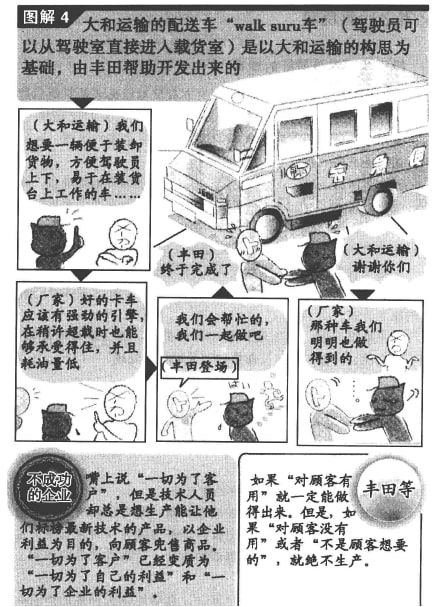
\includegraphics[width=10cm]{丰田p3.jpg}

很多软件公司现在已经开始从以前的瀑布式开发(几个月后才有产品出来),变成敏捷冲刺,每2周便与客户回顾,看是否是他们要的东西。我们QAD的方式基于SCRUM的基础上,也要求客户把需求分成``实体''与``行为''写需求,自动计算功能点数,也帮助开发人员减少误解客户需求。

\hypertarget{ux6807ux6746ux7ba1ux7406-benchmarking}{%
\subsubsection{标杆管理
(Benchmarking)}\label{ux6807ux6746ux7ba1ux7406-benchmarking}}

丰田(如下图)很注重各种标杆,例如内部标杆、竞争性标杆等。软件开发也应该同样利用数据来制定量化目标,例如生产率。最近行业也要求做功能点估算来统一软件报价,有了功能点,团队就可以利用它来衡量软件团队的生产率,它也有不同行业的标杆做参考。


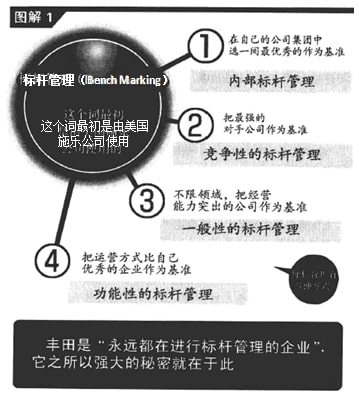
\includegraphics[width=10cm]{丰田p1.jpg}

\textbf{收集每迭代项目数据,建立标杆}\\
我们要求每个迭代项目组都需要提供数据,填进模板中,开始时因公司还没有历史数据的基线,我们就借用行业数据,从下图看到C\#编码的有效率都是很好(绿色)


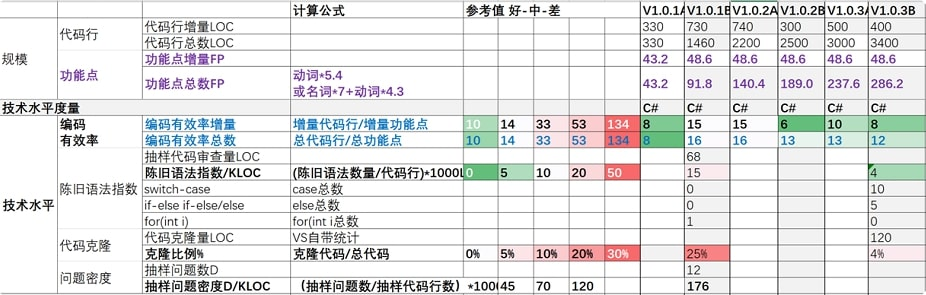
\includegraphics[width=10cm]{陈爱明p15.jpg}

因各项目的数据都会汇总在一个公司级的数据表,每个项目组不仅仅看到自己的表现,也可以看到其他项目组的情况。

建立公司标杆不能单靠数据分析员一个人分析判断,而是应由过程改进组与所有相关项目经理一起讨论:\\
*展示(投影)项目多轮迭代数据

\begin{itemize}
\tightlist
\item
  这些不同项目的数据类似吗?还是差异大,要分开定基线?
\item
  里面有些离散点数据?为什么?
\item
  数据准不准确?合不合理?
\end{itemize}

这样才可以知道数据是否正确,标杆/基线是否适用于项目?

\hypertarget{ux5bb9ux6613ux5b9eux73b0ux7684ux76eeux6807ux4e0dux662fux597dux76eeux6807}{%
\subsubsection{容易实现的目标不是好目标}\label{ux5bb9ux6613ux5b9eux73b0ux7684ux76eeux6807ux4e0dux662fux597dux76eeux6807}}

\begin{itemize}
\tightlist
\item
  不是``削减一成'',而是通过``取消一个零''来发现浪费
\end{itemize}

把原先需要三小时的工作,改用三分钟完成。\\
听到上司这个要求,你该怎么回答呢?多数人会常识性地回答:``这太强人所难了''、``绝对做不到''。\\

\framebox{%
\begin{minipage}[t]{0.97\columnwidth}\raggedright
丰田 {``单分换模(Single Minute Exchange of
Die)''}例子:\\
1965年,丰田汽车在推行丰田生产方式时遭遇一个瓶颈:装置更换时间太长,其中特别是500吨冲压机和1000吨冲压机的模具,更换时间长达2\textasciitilde{}4小时。如果不缩短这两个模具的更换时间,就不可能实现多品种少量生产方式。
\\挑战由大野耐一先生统领,在生产管理的先行者,新乡重夫先生的指导下,分两个阶段展开。\\
改善开始之前,新乡先生凭借自己多年的工作经验,了解到装置更换有两种方式。\\
①内部装置更换------必须在机器停下来以后,才能进行的装置更换。\\
②外部装置更换------能在机器运转过程中,或是在运转起来以后,进行的装置更换。\\
要缩短时间,把内部装置更换和外部装置更换清楚地分开来是一个关键。能在外部装置替换作业中进行的工作,就全部在外部装置替换过程中实施。同时,分别对内部装置替换和外部装置替换进行改善。通过这种方法,装置更换时间缩短为一个半小时。\\
完成这一改善花费了半年时间。通常能有这样的成果就可以告一段落了。但是,大野先生仍要求进一步缩短时间。\\
他要求把更换过程``缩短为3分钟!''通常通过改善能把原先的2\textasciitilde{}4小时缩短为一个半小时,就可以很满意地说``已经很好了''。但是,大野先生不这么想。\\
他认为:``既然能缩短到这个水平,那么继续改善肯定可以把时间缩短为3分钟。''\\
改变汽车生产的单分换模的秘密\\
对于这一要求,在以新乡先生为中心的技术小组中,自然有人提出``3分钟绝对干不完''。但是,新乡先生认为:``如果能把内部装置更换全部转化为外部装置更换,3分钟也不是不可能\\
之后,他着手对多达100个以上的项目进行了改善。\\
首先,进一步对内部装置更换和外部装置更换进行细分,彻底把内部装置更换转化为外部装置更换。同时,想方设法对各种切割工具和模具进行设置,使得更换时用一个动作即可完成。此外,在紧固件上也动了很多脑筋。这样,终于创造出了无数项不花时间、能够简单完成同时可以在作业时保持稳定的改善。\\
紧接着,对作业顺序反复进行改善,实施标准化(制定没有多余工序的作业标准)。这样,在挑战进行了三个月后的某一天,真的只要3分钟就能完成了!这个结果让所有人都大吃一惊。\strut
\end{minipage}}

看下面两个软件项目实例:

\framebox{%
\begin{minipage}[t]{0.97\columnwidth}\raggedright
项目是要更新信息基础平台,团队一直很注重配置管理和模块化设计,为了避免对生产的影响,先做好策划与准备。到了更新时,2位工程师准备新的基线,先本地测好,也准备完整的验收测试包,测试暴露了一些缺陷,先把主要的问题解决,与开发团队讨论后,一致同意进行更新上线。整个更新的过程包括跑完所有自动化测试,在1天内完成。\strut
\end{minipage}}

\framebox{%
\begin{minipage}[t]{0.97\columnwidth}\raggedright
另一个项目是要对一个老系统做修复,这系统已经投产了很多年,希望更新应用服务器的版本。(因为系统本来应用服务器的版本厂家不支持)这个项目最后占用了6个人2个月才能测试好,完成,进入投产。\strut
\end{minipage}}

虽然以上两个项目不是完全一样,但可以看到如果动脑筋,策划好,也能``取消一个零''。\\
例如,我们去年有敏捷团队可以经过6轮冲刺(3个月)把系统缺陷密度减半。

\hypertarget{ux6839ux56e0ux5206ux6790}{%
\subsubsection{根因分析}\label{ux6839ux56e0ux5206ux6790}}

(五个为什么 是一种找根因的方法 , 详见附件B)

\begin{itemize}
\tightlist
\item
  不停留在``原因''上,而要找出``真因'',彻底改善
\item
  不追究责任,而是追究原因\\
\end{itemize}

丰田的大野耐一先生说:

\begin{description}
\tightlist
\item[]
\emph{做到一半是不行的,只有一个期限,``到完成为止''}
\end{description}

当工程师报了有问题就必须要求工程师查找原因、提供数据,但很多时候这个工作并不简单,但大野耐一先生决不放弃,必须找到根因。

我们辅导量化敏捷开发, 每迭代回顾都要收集数据,并做根因分析:
在软件开发,当遗漏到系统测试的缺陷多,便要做讨论,探讨是什么原因?例如:是开发质量问题或测试力度不够,开发的编码有不良习惯,例如拷贝代码,用很大的类等(详见附件A"软件开发质量")。针对代码质量问题,团队便做培训,用新的方式看看会不会有改善?

同样,本来自动化测试的效率在头2、3个迭代都是比较弱(粉红)的,我们与测试人员探讨自动化测试脚本的不足,并针对改善后,后面的迭代就有显著改善(绿)。


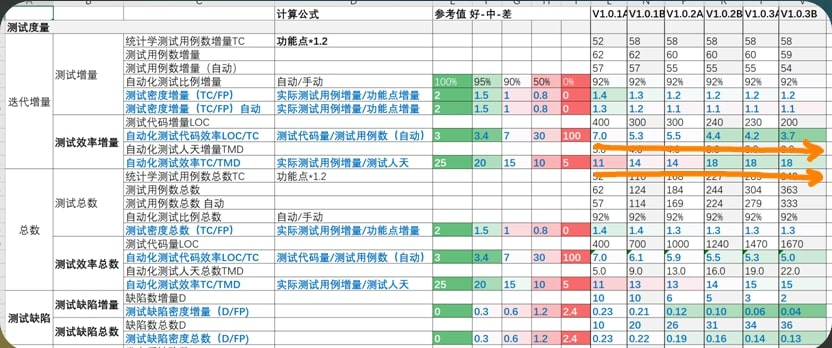
\includegraphics[width=10cm]{陈爱明p17.jpg}

\textbf{预防同类问题再发生}\\
有一家专门做电力的软件公司,它为了加快发布的频率,已经在2年前开始做到每2周自动发布,但他们还是很关注发布的质量,所以发布前都有多轮的审批,确保质量,才允许发布。

如果项目经理赶不上某次发布的,他们就会走一个失效分析
(FMEA),回顾整个过程,哪步出问题?背后什么原因?如何避免同样的问题以后发生。

\hypertarget{ux6210ux957fux6bd4ux6210ux529fux66f4ux91cdux8981}{%
\subsubsection{成长比成功更重要}\label{ux6210ux957fux6bd4ux6210ux529fux66f4ux91cdux8981}}

\begin{itemize}
\tightlist
\item
  要培养人才,``改变体制''比``改变人''更有效
\end{itemize}

有些工厂只依赖张贴标语、海报,希望可以减少工地的事故发生率,但丰田不注重喊口号,而是动手干实事,包括机械保安、设备保安等


\includegraphics[width=10cm]{ft_223_1.jpg}

\framebox{%
\begin{minipage}[t]{0.97\columnwidth}\raggedright
{叫人做之前自己先做一遍给他们看}
本田技研工业在中国创立广州本田的时候,派往当地的都是即将退休的经验丰富的中高年龄层技术人员,这批技术人员成为了厂里的中坚力量。正因为他们的努力,广州的本田工程才获得了成功。\strut
\end{minipage}}

软件开发如何确保质量?比如一个团队有些新人,绝不能简单分派任务,让他自己随意写代码,组长要先想好整个架构,主要有哪些类,之间有什么关系,每个方法和类要注释说明,然后分配给新手去执行,避免事后返工。学校里编码练习也不会只描述需求,通常会指出需要那些类、方法,有什么作用,防止学生走偏。

但软件开发人员的能力有高低之别,如何让新手可以跟高手有效学习呢?代码评审其实是很有效的培训,比单靠讲课更有效。我们会建议团队按高手的时间来安排评审,让新手从中学习。不一定预定在哪天哪时,以便减少对高手时间安排的影响(他时间宝贵),也能取得培训效果。

\hypertarget{ux6240ux6709ux4ebaux53c2ux4e0eux6539ux8fdb}{%
\subsubsection{所有人参与改进}\label{ux6240ux6709ux4ebaux53c2ux4e0eux6539ux8fdb}}

\framebox{%
\begin{minipage}[t]{0.97\columnwidth}\raggedright
{带诚意去赢得协作}
B先生所在的A公司曾以丰田生产方式为基础进行了生产改革。\\
要进行生产改革没有技术部门的配合是行不通的。但是,任凭
B先生怎么要求,技术部门依然毫不合作。B先生实在没有办法了,只能向总裁要求:
``请加大我手上的权力,让我可以支配技术部。''总裁回答:
``你去给我请教了大野(耐一)先生以后再说!''\\
于是B先生去找大野先生,在听他诉说了自己面临的窘境以后,大野先生对他说:
``你这一两天跟我一起去工厂转转吧!''并于百忙之中抽出时间带B先生参观了丰田的工厂以及附近的协作企业的工厂。这期间,大野先生什么话都没说,只在第二天下午问B先生:``怎么样,你明白了吗?''\\
B先生回答:
``我觉得在工厂听到的关于厂长的改善事例,跟丰田方式所强调的重点好像不太一致。''听了B先生的回答以后,大野先生点头:
``就连我,也是一直都在忍耐的啊。工作并不是有权力就能解决问题的。要想得到对方的理解和信任,拿出诚意去找人家吧。''\\
从那以后,
B先生再也不找``因为我手里没有权力''之类的借口,而总是带着诚意去找对方协商,不久以后,他成功地对A公司实施了生产改革。\\
每当听到有人感慨``下属不听话''的时候,一位曾在丰田工作的人就会说:
``你要求自己的孩子"每天学习三小时'时,他会听话去学习吗?''\\
对方的回答是:
``估计没用。''\\
``连自己的孩子都这样,更何况那些成年的员工呢?''\strut
\end{minipage}}

我们开始要求企业拿出试点项目来做量化敏捷开发(QAD)时,阻力也很大,我们只好挑一些愿意并有能力的先锋团队。过了几个月后,其他本来观望的项目组看到确实有效,也愿意加入。所以在公司推动过程改进必须先试点后推广。

因为与以往的做法截然不同,必须经历:\\
学习 - 尝试 - 学习 - 尝试执行\\
不断循环才开始把握。 团队也会问老师收集了几轮数据了。不知道有什么用处?
但我们不直接给答案,而是重新提醒他们各种学过的分析技巧与方法,让他们自己尝试找答案。

反过来,如果团队没有经历这个过程,只遵循老师制定的一套固定方法,项目组很可能评估过后,便恢复以前,不能持续。

推动量化敏捷开发也一样,不能单依赖一套固定方法,我们利用CMMI量化管理的实践重点,例如量化目标、度量可操作定义、基线预测模型等。首先教他们用简化功能点,使每个团队都有可比的规模大小基数,然后让他们收集每一迭代的缺陷数,工作量和一些可控因素,引导他们如何分析这些迭代数据,制定本项目的下一迭代的量化目标。
虽然我们会提供一些统计分析的技巧,给他们参考,但是还靠项目经理与团队自己讨论,看用什么方式达到量化项目管理的要求。

\hypertarget{ux603bux7ed3}{%
\section{总结}\label{ux603bux7ed3}}

这3篇"再读德鲁克",从信息化挑战开始,我们探讨管理者应如何做好数字化、智能化管理,收集哪些数据,帮助企业管理。然后我们再回顾有哪些方法,可以帮助知识工作者提高效率和质量。这篇我们从管理外包的问题开始,引申到丰田生产方式的一些案例,了解管理者的"系统"。

丰田故事让我们看到``系统''如何帮公司培养知识工作者,发挥人的无限智慧,
为公司增值。\\
汽车制造大部分利用自动化机器,但当今软件开发生产和质量,
非常依赖开发人员的水平, 所以我们更需要建立``系统'',帮助员工快速成长。

前面分享的九个丰田管理思路,其实都能在软件产品开发用上:

\begin{enumerate}
\tightlist
\item
  以忙碌为耻
\item
  培养人才 - 逼他们动脑筋
\item
  从心里相信``大家的力量''
\item
  不以``我们公司''作主语
\item
  标杆管理 (Benchmarking)
\item
  容易实现的目标不是好目标
\item
  根因分析
\item
  成长比成功更重要
\item
  所有人参与改进
\end{enumerate}

在互联网年代,数字化管理已经不是未来,在软件产品开发,很多公司已经从以往的瀑布型开发模式转为敏捷开发,以便更好反应客户的需求变化,也让团队效率提升到极限。

2周一冲刺比以往几个月才完成一个项目,本应可以收集十倍的数据(假如项目平均5个月),但碍于敏捷方法缺乏一套度量标准,公司无法形成基线
/ 标杆。

4年前,我们开始为企业推动量化敏捷开发(QAD),团队就可以基于功能点的生产率与质量基线,并在6
- 9个月时间,利用对可控因子的根因分析,可以把缺陷率减半。

从我们过去三年,针对那些已经使用敏捷SCRUM开发的软件开发公司,辅导团队提升到量化敏捷开发,
但管理层千万不要以为这个改变过程轻松、 快速。正好相反,
任何文化的改变都会遇到很大阻力,但只要管理深信必需建立这个``系统'',破釜沉舟,才有希望成为大陆软件开发未来的``丰田''!

\hypertarget{ux53cdux9988}{%
\section{反馈}\label{ux53cdux9988}}

\framebox{%
\begin{minipage}[t]{0.97\columnwidth}\raggedright
上海一总监问: "可否说明一下市面流行的敏捷开发(如 SCRUM ) , 如何分配任务
, 有那些方法?"\strut
\end{minipage}}

敏捷一般建议基于I.N.V.E.S.T.原则把需求分解成用户故事。

\begin{description}
\tightlist
\item[]
Independent (from other user stories)

Negotiable (on how to implement)

Valuable (for customers)

Estimable

Small (to complete in a Sprint)

Testable
\end{description}

但具体怎么分每个人可能有不同的想法,而且用故事点 估计规模大小,
但故事点只是项目组自己的定义,不同团队间无法比较,难以利用各项目度量数据,建立公司标杆(基线)。

针对以上不足, 也方便开发/测试能与需求打通,
和团队使用功能点作为规模,估算工作量 / 工期。

我们会教团队按场景(Scenario) 、 实体(Entity) ,行为(Activity)写需求。
以便与开发工作 / 测试工作对应。\\
(实例 ,注: 实体浅蓝色,有框)


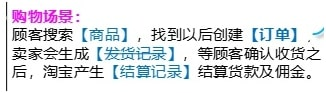
\includegraphics[width=10cm]{场景1.jpg}

团队便容易把与行为对应的开发任务,按优先级,安排到各冲刺中。
测试人员也可以从而估算出测试用例数,测试工作量,甚至缺陷数范围。
敏捷团队从定性管理,升到定量管理。


\cite{drucker3References1}
\cite{drucker3References2}



